\section{Методы приближения функций. Численное дифференцирование и интегрирование}

\subsection{Постановка задачи}
3.1. Используя таблицу значений $Y_i$ функции $y=f(x)$, вычисленных в точках $X_i, i=0,\cdots,3$ построить интерполяционные многочлены Лагранжа и Ньютона, проходящие через точки ${X_i, Y_i}$.  Вычислить значение погрешности интерполяции в точке $X^*$.

{\bfseries Вариант:} 19
    \begin{equation}
        y = arcsin(x) + x
    \end{equation}
    a)
    \begin{equation}
        X_i = -0.4, -0.1, 0.2, 0.5
    \end{equation}
    б)
    \begin{equation}
        X_i = -0.4, 0, 0.2, 0.5
    \end{equation}
    \begin{equation}
        X^* = 0.1
    \end{equation}
\pagebreak

\subsection{Результаты работы}
\begin{figure}[h!]
\centering
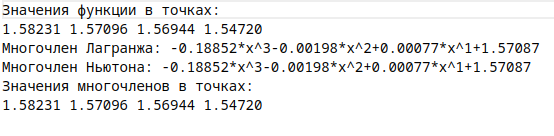
\includegraphics[width=.5\textwidth]{lab3.1}
\caption{Вывод в консоли}
\end{figure}


\subsection{Исходный код}
\lstinputlisting[title=\texttt{Lab3.1.cpp}]{../stud/saifullin/task3.1/Lab3.1.cpp}
\pagebreak

